\documentclass[conference]{IEEEtran}
%\IEEEoverridecommandlockouts

\usepackage{amsmath,amssymb,amsfonts}
\usepackage{algorithmic}
\usepackage{graphicx}
\usepackage{textcomp}
\usepackage{xcolor}
\usepackage{biblatex}

\graphicspath{ {./img/} }

\def\BibTeX{{\rm B\kern-.05em{\sc i\kern-.025em b}\kern-.08em
    T\kern-.1667em\lower.7ex\hbox{E}\kern-.125emX}}

\addbibresource{document.bib}

\begin{document}

\title{Security in WebRTC Peer-To-Peer connections and knowing who you're talking to\\
}

\author{\IEEEauthorblockN{Marc André Matija}
\IEEEauthorblockA{\textit{info@casqan.net}} \\
\textit{}
}

\maketitle

\begin{abstract}
\end{abstract}

\begin{IEEEkeywords}
peer-to-peer, WebRTC
\end{IEEEkeywords}

\section{Introduction}
In recent years, the proliferation of real-time applications such as video conferencing, online collaboration tools, multiplayer gaming, 
and decentralized content-sharing platforms has brought Peer-to-Peer (P2P) communication technologies to the forefront of modern web 
infrastructure. At the heart of this evolution lies Web Real-Time Communication (WebRTC), a framework that enables seamless audio, video,
and data exchange directly between devices without relying on centralized servers for data transmission. WebRTC's integration into browsers and 
its adoption in applications like Google Meet, Zoom, and Discord have cemented its position as a cornerstone of real-time communication on the web.
The importance of P2P technologies stems from their inherent advantages over the traditional server-client model. By enabling direct communication 
between peers, P2P systems reduce the dependency on centralized servers, thereby lowering costs, improving scalability, and reducing latency. % Citation needed
These characteristics make P2P well-suited for scenarios requiring high performance and efficiency, such as low-latency video conferencing 
and large-scale decentralized networks. Additionally, as edge computing and decentralized ecosystems, including blockchain technologies, continue 
to grow, P2P communication is poised to play a critical role in shaping the future of the web.
However, the adoption of P2P technologies 
introduces unique security challenges that differ fundamentally from the established server-client architecture. In the server-client model,
security largely revolves around protecting a central server, with mechanisms such as TLS ensuring secure communication between clients and
the server. In contrast, P2P systems require trust to be established directly between endpoints, often in dynamic and transient network 
environments. This shift necessitates the use of mechanisms like end-to-end encryption, peer authentication, and data integrity validation to
ensure secure interactions without the intermediary role of a central authority. Additionally, P2P architectures must contend with new vectors
of attack, such as man-in-the-middle attacks during peer discovery, unauthorized data relay via TURN servers, and exploitation of NAT traversal
mechanisms like STUN. This paper explores the growing relevance of WebRTC and P2P technologies in modern web infrastructure, with a focus on 
their security implications. It delves into the distinctions between P2P and server-client security models, highlights the challenges of ensuring 
authentication, integrity, and authenticity in P2P systems, and examines the mechanisms employed by WebRTC to address these challenges. By doing so, 
this paper aims to shed light on the critical role of security in advancing the adoption and reliability of P2P technologies in the modern web.

\section{What WebRTC does and how it works}
WebRTC is a web standard that facilitates a peer-to-peer connection between browsers or native clients. In order to do so, a WebRTC connection 
is required, which involves several steps to enable secure peer-to-peer communication for audio, video, and data. 
The process begins with signaling, where peers exchange Session Description Protocol (SDP) messages and ICE candidates via a 
signaling server (e.g., WebSocket or SIP). These exchanges negotiate media codecs, encryption keys, and network details. \cite{W3C_WebRTC}

To traverse NATs and firewalls, WebRTC uses the ICE framework, leveraging STUN servers to discover public IP addresses and ports. 
When direct connections are blocked by restrictive networks, TURN servers relay traffic to ensure connectivity. After signaling, a
DTLS handshake is performed to exchange cryptographic keys securely. These keys are then used by SRTP to encrypt audio and video streams, 
ensuring confidentiality and integrity. \cite{W3C_WebRTC}

Once these steps are complete, a direct peer-to-peer connection is established, with audio/video transmitted over SRTP 
and other data over SCTP. This process relies on key components like signaling servers, STUN/TURN servers, and browser-supported 
WebRTC APIs to ensure seamless, secure communication across various network conditions. \cite{W3C_WebRTC}

From a security standpoint, an important part is the Session Description Protocol (SDP) handshake. A critical component of the WebRTC signaling process, 
enabling two peers to negotiate media parameters and establish a secure connection.\cite{RFC8827} While SDP itself is a plain-text protocol 
and does not provide security features, it plays a pivotal role in enabling the secure setup of WebRTC sessions by facilitating the exchange 
of cryptographic keys, network information, and supported capabilities. A robust security architecture around SDP ensures the integrity, 
authenticity, and confidentiality of the WebRTC session.

Key Components of the SDP Handshake in WebRTC
\begin{itemize}
    \item \it{Offer/Answer Model:} The handshake begins with one peer generating an SDP "offer" that contains information about supported media codecs, network candidates 
    (IP addresses and ports), and cryptographic keys for media encryption. The receiving peer responds with an SDP "answer" that finalizes 
    the agreed-upon parameters. This process is governed by the RFC 3264.
    \item \it{ICE Candidates:} The SDP offer/answer exchanges Interactive Connectivity Establishment (ICE) candidates, which include potential connection 
    endpoints. These candidates are necessary for traversing NATs and firewalls using STUN/TURN servers.
    \item \it{DTLS Fingerprints:} A critical security component in the SDP handshake is the inclusion of DTLS fingerprints—hashes of the public keys used during
    the subsequent DTLS handshake. These fingerprints ensure that peers can verify the authenticity of the DTLS certificates exchanged 
    later, preventing man-in-the-middle (MITM) attacks during key negotiation.
    \item \it{Key Exchange:} SDP facilitates the secure exchange of cryptographic keys used by Secure Real-time Transport Protocol (SRTP) for encrypting 
    media streams. WebRTC uses DTLS-SRTP to derive encryption keys during the DTLS handshake, ensuring that media streams remain 
    protected from eavesdropping and tampering.
\end{itemize}

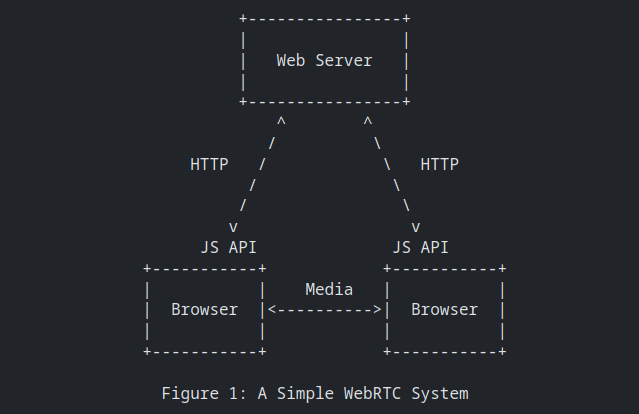
\includegraphics[width=0.45\textwidth]{WebRTC basic Structure}

Unlike most conventional real-time systems (e.g., SIP-based [RFC3261] soft phones), WebRTC 
communications are directly controlled by some Web server, via a JavaScript (JS) API as shown in Figure 1.

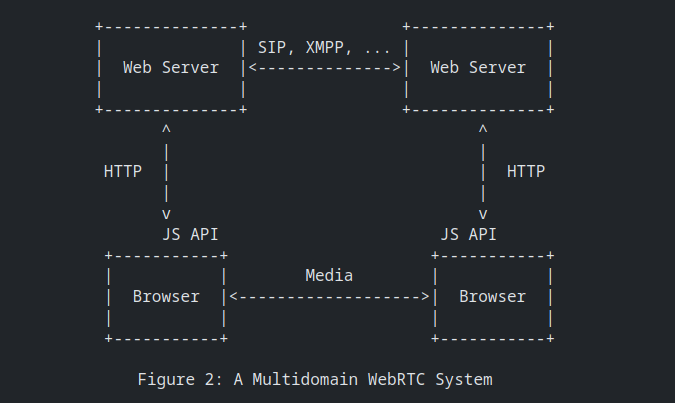
\includegraphics[width=0.45\textwidth]{multi domain calling.png}
A more complicated system might alow for inter-domain calling, as shown in Figure 2. The protocol to be used between the domains 
is not standardized by WebRTC, requires other form of security and may rely on other standardized Protocols such as the
Session initiation Protocol (SIP), or Extensible Messaging and Presence Protocol (XMPP). \cite{RFC8827}

\section{Authentication in WebRTC}
\subsection{Trust Model}

The basic assumption of the standardized architecture as in RFC[8827]\cite{RFC8827} is that network resources exist in a hierarchy of trust, rooted in the browser, 
which serves as the user's Trusted Computing Base (TCB). Any security property which the user wishes to have enforced must be 
ultimately guaranteed by the browser (or transitively by some property the browser verifies). Conversely, if the browser is 
compromised, then no security guarantees are possible. Note that there are cases (e.g., Internet kiosks) where the user can't 
really trust the browser that much. In these cases, the level of security provided is limited by how much they trust the browser.
Optimally, we would not rely on trust in any entities other than the browser. However, this is unfortunately not possible 
if we wish to have a functional system. Other network elements fall into two categories: those which can be authenticated by 
the browser and thus can be granted permissions to access sensitive resources, and those which cannot be authenticated and 
thus are untrusted.

\subsection{Authenticated Entities}
There are two major classes of authenticated entities in the system:
\begin{itemize}
    \item Calling services: Web sites whose origin we can verify (optimally via HTTPS, but in some cases because we are on a topologically restricted 
    network, such as behind a firewall, and can infer authentication from firewall behavior).
    \item Other users: WebRTC peers whose origin we can verify cryptographically (optimally via DTLS-SRTP).
\end{itemize}

Note that merely being authenticated does not make these entities trusted. For instance, just because we can verify that 
<https://www.example.org/> is owned by Dr. Evil does not mean that we can trust Dr. Evil to access our camera and microphone. 
However, it gives the user an opportunity to determine whether they wish to trust Dr. Evil or not; after all, if they desire to 
contact Dr. Evil (perhaps to arrange for ransom payment), it's safe to temporarily give them access to the camera and microphone 
for the purpose of the call, but they don't want Dr. Evil to be able to access their camera and microphone other than during the 
call. The point here is that we must first identify other elements before we can determine whether and how much to trust them.
 Additionally, sometimes we need to identify the communicating peer before we know what policies to apply.

\subsection{Unauthenticated Entities}
Other than the above entities, we are not generally able to identify other network elements; thus, we cannot trust them. 
This does not mean that it is not possible to have any interaction with them, but it means that we must assume that they will 
behave maliciously and design a system which is secure even if they do so.


\section{Identification in WebRTC}
"On the internet, no one knows you are a dog", the punchline of a comic by Peter Steiner back in 1993.
More than 20 years later, assurance of user identity remains a challenge, and user impersonations are
more frequent. \cite{User_Identity_for_WebRTC_Services_A_Matter_of_Trust} However, identification in 
Peer-To-Peer systems becomes a big problem, as a peer has to trust, that a connecting peer is who he 
pretends to be. In the standard HTTPs environment the ssl
protocol is used to facilitate a trusted connection from client to server, in which the Server
has been previously verified by a Certificate Authority, which is trusted by the client. 
In a general sense, this means that two peers require a third trusted party to facilitate
identification in a secure manner.\cite{RFC8827} This part could be a peer, or superpeer that has been previously verified
by the opposing party and himself\cite{Security_Mechanisms_for_Signaling}.

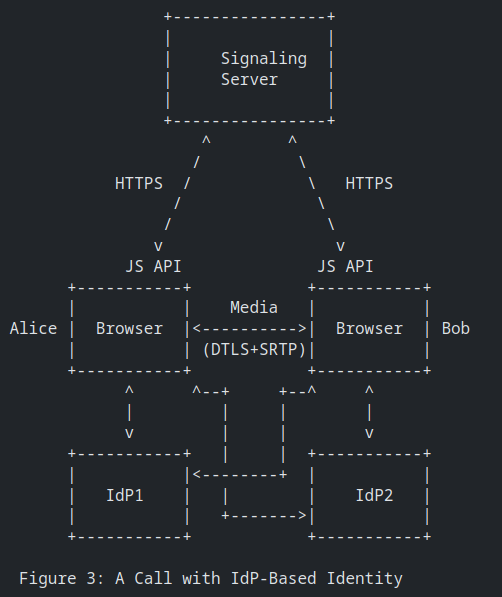
\includegraphics[width=0.45\textwidth]{call with IdP Based Identity.png} % remake as SVG

\subsection{IdP}
As a standardized way, WebRTC offers and answers (and hence the channels established by
RTCPeerConnection objects) can be authenticated by using a web-based Identity
Provider (IdP). The idea is that the entity sending an offer or answer acts as the
Authenticating Party (AP) and obtains an identity assertion from the IdP which it
attaches to the session description. The consumer of the session description (i.e.,
the RTCPeerConnection on which setRemoteDescription is called) acts as the
Relying Party (RP) and verifies the assertion.\cite{WebRTC_Identity}

In order to verify assertions, the IdP domain name and protocol are taken from the
domain and protocol fields of the identity assertion.

Communication with the IdP is established by the user agent loading the IdP JavaScript from
the IdP. The URI for the IdP script is a well-known URI formed from the “domain”
and “protocol” fields, as specified in \cite{RFC8827}.
The IdP MAY generate an HTTP redirect to another "https" origin, the browser
MUST treat a redirect to any other scheme as a fatal error.
The user agent instantiates an isolated interpreted context, a JavaScript realm that
operates in the origin of the loaded JavaScript. Note that a redirect will change the
origin of the loaded script. The realm is populated with a global that implements both the
RTCIdentityProviderGlobalScope and WorkerGlobalScope [WEBWORKERS] interfaces.
The user agent provides an instance of RTCIdentityProviderRegistrar named
rtcIdentityProvider in the global scope of the realm. This object is used by the IdP to
interact with the user agent.

\section{Authenticity and Data Integrity}
WebRTC at it's core uses User Datagram Protocol a lightweight, connectionless communication protocol 
within the Internet Protocol (IP) suite, defined in [RFC 768]. It enables applications to send and receive 
discrete packets of data, known as datagrams, without requiring a prior connection. While UDP, does
include a checksum to verify it's data integrity, it does not include any standard specification for ensuring
packages have been received by the opposing party, relying on protocol extensions to facilitate save
data transmission. \cite{RFC768}
WebRTC enforces end-to-end encryption for all media and data streams by default, using 
standards like DTLS for signaling and data channels while relying on SRTP for media transmission. \cite{RFC8826}

\subsection{DTLS}
The DTLS protocol is a cryptographic protocol designed to provide secure communication over unreliable datagram-based 
transport layers such as UDP. It is defined in RFC 6347 and serves as an adaptation of the widely used Transport 
Layer Security (TLS) protocol, which secures communication over connection-oriented transport protocols like TCP. 
By incorporating mechanisms to handle packet loss, reordering, and duplication, DTLS ensures secure, reliable 
communication in real-time and low-latency scenarios.\cite{RFC6347}

*insert technical description of DTLS*

\subsection{SRTP}
The Secure Real-time Transport Protocol (SRTP) is a security extension of the Real-time Transport Protocol (RTP), 
designed to provide encryption, message authentication, and integrity for real-time multimedia communication. 
Introduced in 2004 and defined in RFC 3711, SRTP ensures the confidentiality and integrity of voice, video, and 
other real-time data transmitted over potentially insecure networks, such as the internet. \cite{RFC3711}

*insert description of SRTP*

\section{Risks and Concerns}
\subsection{WebRTC Leaks}
Even tho standardized and widely adopted, WebRTC's security is not bulletproof. 
Highlighted in the paper One leak will sink the ship, due to it's inherent nature 
of establishing a Peer-To-Peer connection, WebRTC requires
knowledge about a peers ip address, this could cause the potential leak of someone's location, even with
the use of VPN's. Possible leaked information can include the users 
\begin{itemize}
    \item \it{Public IPv6 address} this is the IPv6 address of the
    platform and is typically assigned by the ISP of the client.
    \item \it{Public Temporary IPv6 address:} this address is assigned
    by the network to which the client platform is attached.
    \item \it{Unique local address (ULA) assigned by LAN:} this IPv6
    address is assigned by the network to which the client
    platform is attached, and is the approximate IPv6 counterpart of 
    the Private IPv4 address assigned by LAN [5].
    \item \it{Private IP address assigned by the VPN server:} this pri-
    vate (IPv4 or IPv6, depending on the VPN configuration)
    address is assigned by the VPN server.
    \item \it{Private IPv4 address assigned by LAN:} this address is 
    assigned by the network to which the client platform is
    attached.
  \end{itemize}\cite{One_leak_will_sink_a_ship}
While not all of these are worth the same, a public IPv6 Address leak for example, is more dangerous than a
Unique local Address leak, these are still security concerns VPNs try to solve.
VPN providers have now setup WebRTC address leak detectors to inform the user, if a leak of their private IP address
is present. Providers for these Services include some of the major players in the private VPN space, such as 
ExpressVPN and SurfShark. % https://www.expressvpn.com/webrtc-leak-test 
Some solutions to this problem include:

\begin{itemize}
    \item Disabling WebRTC entirely inside the Browser or connecting client.
    \item Disabling IPv6 to reduce the amount of information leaked, if a leak occurs.
    \item Relying on Relay Server to transmit data to a central location before continuing on to the connected peer,
    which however, does need to be implemented by the Developers of the application using WebRTC, which defeats the
    purpose of not having a central server in peer-to-peer to begin with.
\end{itemize}\cite{One_leak_will_sink_a_ship}
However, all these are mere workarounds and WebRTC without VPNs has to inherently leak
IP addresses as they are required to connect to another peer.

\subsection{Man-In-The-Middle during signaling}
WebRTC's peer by default require End-To-End Encryption \cite{RFC8827}, however during the signaling process,
it is susceptible to Man in the middle attacks \cite{Security_Mechanisms_for_Signaling}

\section{Conclusion}

\printbibliography{}

\end{document}